%!TeX program = xelatex
\documentclass[12pt,a4paper,UTF8]{ctexart}
\usepackage{swjtuReport}

% 将一级标题改成“第1章”,若\arabic改成\chinese即为“第一章”
% \usepackage{titletoc}
% \ctexset{section={name={第,章},number={\arabic{section}}}}   

\begin{document}
%%------------------------------封面------------------------------%%
\cover
\thispagestyle{empty} % 首页不显示页码
%%------------------------------摘要------------------------------%%
% \newpage
% \pagenumbering{Roman} % 重新计算页码,并将摘要、目录的页码设置成罗马数字页码

% \begin{abstract}\normalsize   % 更改摘要的内容的字体大小

% 在此填写摘要的内容。

% \noindent \textbf{关键词:}
% 关键词1;关键词2;关键词3;关键词4

% \end{abstract}
%%------------------------------目录页----------------------------%%
\newpage
\pagenumbering{Roman} % 重新计算页码,并将摘要、目录的页码设置成罗马数字页码
\begin{center}
    \tableofcontents
\end{center}
%%------------------------------正文------------------------------%%
\newpage
\pagenumbering{arabic} % 重新计算页码,并将正文的页码设置成阿拉伯数字页码

\section{设计要求}
设计普通型弹簧压力表,其技术要求为:
\subsection{测量范围}
测量下限制为0,测量上限制为:6。单位为MPa(${\approx}10kgf/cm^2$)
\subsection{精度等级}
精度等级:1.5级
\subsection{外形尺寸}
外形尺寸如\autoref{figure1.1}所示:
\begin{figure}[!htbp]
    \centering
    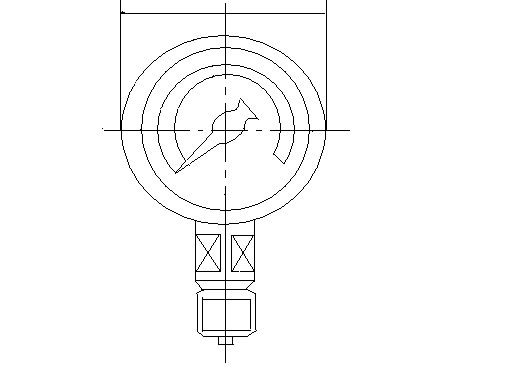
\includegraphics[width =0.45\textwidth]{figures/1.1.1.png}
    \caption{}
\end{figure}
\begin{figure}[!htbp]
    \centering
    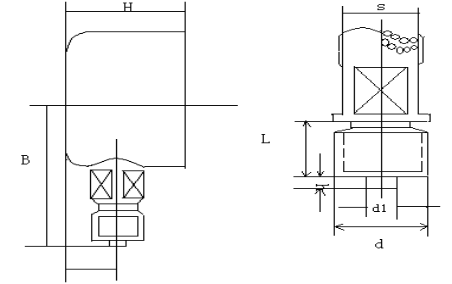
\includegraphics[width =0.65\textwidth]{figures/1.1.2.png}
    \caption{表壳外形尺寸}
    \label{figure1.1}
\end{figure}
\newline
接头位置为径向;表壳无边;表壳公称直径D=100mm;$H{\le}60mm$,
\begin{equation}
{B{\le}100mm,a=M20{\times}1.5,S=17_{-0.28}^{\circ},\\L=20_{{\pm}0.52},h=5_{{\pm}0.30},d_{1}=6_{-0.30}}\nonumber
\end{equation}
\subsection{标尺特性}
等分分度;标度角:$270^{\circ}$;
\begin{table}[!htbp]
    \centering
\caption{测量上限值与最小分度值的关系}
\label{tab:1.1}
    \begin{tabular}{|c|c|c|c|c|c|c|} \hline 
         测量上限值&0.06&0.1&0.16&0.25&0.4&0.6\\ \hline 
         测量下限值&0.001&0.002&0.005&0.005&0.01&0.01\\ \hline 
         测量上限值&1&1.6&2.5&4&0.6& \\ \hline 
         测量下限值&0.02&0.05&0.05&0.1&0.1& \\ \hline
    \end{tabular}
\end{table}
\newline

由\autoref{tab:1.1},由于我们设计的压力表量程上限为0.4Mpa,所以选择最小分度值为0.01.所以,所设计的压力表最小分度值为0.01MPa(${\approx}10kgf/cm^2$)

\section{设计方案}

\subsection{弹簧管}

\subsection{曲柄滑块机构}

\subsection{齿轮传动}

\subsection{游丝}

\subsection{标尺指针}

\section{测量环节的参数选择与计算}
\subsection{弹簧管}
\subsection{弹簧管的强度校验}
\subsection{齿轮传动机构}
\subsection{曲柄滑块机构}
\subsection{齿轮机构设计}
\subsection{表盘的设计}
\subsection{指针的设计}
\subsection{轴承的设计}
\subsection{游丝的设计}
\section{仪器非线性设计误差计算}
\section{结论}
\section{模板说明}
本模板主要适用于一些课程的平时论文以及期末论文,默认页边距为2.5cm,中文宋体,英文Times New Roman,字号为12pt(小四)。

编译方式:\verb|xelatex -> bibtex -> xelatex*2|


默认模板文件由以下四部分组成:
\begin{itemize}
    \item \texttt{main.tex} 主文件
    \item \texttt{reference.bib} 参考文献,使用bibtex
    \item \texttt{swjtuReport.sty} 文档格式控制,包括一些基础的设置,如页眉、标题、姓名等
    \item \texttt{figures} 放置图片的文件夹
\end{itemize}

第一次使用时需前往\texttt{swjtuReport.sty} 对标题、姓名、学号、院所、页眉等进行设置,设置完后即可一劳永逸,封面logo亦可替换

默认带有封面页以及目录页,页码从目录页开始
\section{一些插入功能}
\subsection{插入公式}
行内公式$v-\varepsilon+\phi=2$。

插入行间公式如\autoref{Euler}:

\begin{eqnarray}
\varphi^{\prime} & = & {tg}^{-1} \frac{1-\cos \gamma+\frac{f \times \gamma \times \cos \mu}{R}}{\gamma-\sin \gamma-\frac{f \times \gamma \times \sin \mu}{R}} \label{Euler}\\& = & {tg}^{-1} \frac{1-\cos 250^{\circ}+\frac{5.2 \times 4.3633 \times \cos 12^{\circ}}{34.45}}{4.3633-\sin 250^{\circ}-\frac{5.2 \times 4.3633 \times \sin 12^{\circ}}{34.45}}\nonumber\\ & = & 21.07^{\circ}\nonumber
\end{eqnarray}

\begin{equation}
    f(x) =  {\begin{cases}  x, & x<3 \\  2x, & x=3 \\  4x, & x>3  \end{cases}}\label{方程组}
\end{equation}


\subsection{插入图片}
SWJTU校徽如\autoref{SWJTU}所示,注意这里使用了\verb|~\autoref{}|命令,也就是会自动生成“图”“式”等前缀,无需手动输入。

\begin{figure}[!htbp]
    \centering
    
\includegraphics[width =0.4\textwidth]{figures/swjtu_logo2.pdf}
    \caption{西南交通大学}
    \label{SWJTU}
\end{figure}

插入上面图片的代码:

\begin{verbatim}
    \begin{figure}[!htbp]
        \centering
        \includegraphics[width =0.4\textwidth]{figures/ucas_logo.pdf}
        \caption{西南交通大学}
        \label{SWJTU}
    \end{figure}
\end{verbatim}

\subsection{插入文本框}
本模板定义了一个圆角灰底的文本框,使用简化命令\verb|\tbox{}|即可,如果你不喜欢,可以前往 \texttt{swjtuReport.sty}对其进行修改。

\tbox{
    这是一个圆角灰底的文本框
}

\subsection{插入表格}
本模板文件如\autoref{doc}所示。
\begin{table}[!htbp]
    \centering
    \begin{tabular}{l|l}
    \hline
        文件名 & 说明 \\
        \hline
        \texttt{main.tex}  & 主文件 \\
        \texttt{references.bib} & 参考文献 \\
        \texttt{swjtuReport.sty}  & 文档格式控制\\
        \texttt{figures}  & 图片文件夹 \\
        \hline
    \end{tabular}
    \caption{本模板文件组成}
    \label{doc}
\end{table}

\subsection{插入数学逻辑环境}

\begin{Theorem}   % 定理
\end{Theorem}

\begin{Lemma}   % 引理
\end{Lemma}

\begin{Corollary}   % 推论
\end{Corollary}

\begin{Proposition}   % 命题
\end{Proposition}

\begin{Definition}   % 定义
\end{Definition}

\begin{Example}   % 例
\end{Example}

\begin{proof}   %证明
\end{proof}

\subsection{插入参考文献}
直接使用\verb|\cite{}|即可。

例如:

   \textit{ 此处引用了文献\cite{0Isaac}。此处引用了文献\cite{2016The}}

引用过的文献会自动出现在参考文献中。
\section{写在最后}
\subsection{发布地址}
\begin{itemize}
    \item Github: 
    \url{https://github.com/Pungjay/swjtuReport}
    \item Overleaf:  \url{https://cn.overleaf.com/latex/templates/swjtureport/drdffmpsxsbc}
\end{itemize}

%%------------------------------参考文献---------------------------%%
\newpage
\reference
\addcontentsline{toc}{section}{参考文献}   % 将参考文献作为一级标题加入到目录

\end{document}